\documentclass[conference]{IEEEtran}
\IEEEoverridecommandlockouts

\usepackage{cite}
\usepackage{amsmath,amssymb,amsfonts}
\usepackage{algorithmic}
\usepackage{graphicx}
\usepackage{textcomp}
\usepackage{xcolor}
\usepackage{booktabs}
\usepackage{hyperref}

\def\BibTeX{{\rm B\kern-.05em{\sc i\kern-.025em b}\kern-.08em
    T\kern-.1667em\lower.7ex\hbox{E}\kern-.125emX}}

\begin{document}

\title{GNN-DQN: A Graph Neural Network Deep Q-Network Agent for
Centrality-Guided Routing in Opportunistic Networks}

\author{
\IEEEauthorblockN{Gopu Devi Saranya}
\IEEEauthorblockA{\textit{Dept. of Computer Science} \\
\textit{SRM University AP}\\
Andhra Pradesh, India}
\and
\IEEEauthorblockN{Aluru Ganesh Reddy}
\IEEEauthorblockA{\textit{Dept. of Computer Science} \\
\textit{SRM University AP}\\
Andhra Pradesh, India}
\and
\IEEEauthorblockN{I.V.G. Harsha Vardhan}
\IEEEauthorblockA{\textit{Dept. of Computer Science} \\
\textit{SRM University AP}\\
Andhra Pradesh, India}
\and
\IEEEauthorblockN{Dr. Ch. Anil Carie}
\IEEEauthorblockA{\textit{Dept. of Computer Science} \\
\textit{SRM University AP}\\
Andhra Pradesh, India}
}

\maketitle

\begin{abstract}
Routing in opportunistic networks — characterized by intermittent
connectivity and the absence of stable end-to-end paths — demands
adaptive strategies that go beyond static centrality heuristics.
We propose GNN-DQN, a routing agent that combines a two-layer
Graph Convolutional Network (GCN) encoder with a Deep Q-Network
(DQN) policy to jointly learn structural and dynamic network
features. Evaluated on a 50-node weighted network simulator across
10 independently generated topology instances, GNN-DQN achieves a
mean Packet Delivery Ratio (PDR) of $70.6\% \pm 11.33\%$,
outperforming the strongest baseline (Random Forest: $60.8\% \pm
6.68\%$) by 9.8 percentage points (10-seed). However, an ablation
study reveals that a plain DQN significantly outperforms GNN-DQN
on these fixed topologies (88.7\% vs 70.6\%, $p=0.0098$),
indicating that global mean pooling dilutes node-specific routing
signals. A secondary ablation restricting both models to strictly
local state features (removing global centrality inputs) further
confirms this liability, with the Plain DQN achieving 96.0\% PDR
compared to GNN-DQN's 84.0\%. A preliminary evaluation on a single
unseen 80-node topology yields 73\% PDR, though both models share
a fixed 50-action output layer, requiring future architectural
changes to validate true structural generalization. On a single
representative evaluation run, GNN-DQN reduces average hop count
to 2.0, versus 16--18 hops for all other methods.
\end{abstract}

\begin{IEEEkeywords}
opportunistic networks, centrality routing, graph neural network,
deep Q-network, reinforcement learning, relay selection
\end{IEEEkeywords}

\section{Introduction}

Opportunistic networks operate in environments where stable
end-to-end paths are unavailable due to node mobility, link
failures, or sparse deployment. Examples include disaster-response
coordination networks, vehicular ad-hoc networks (VANETs), and IoT
sensor meshes in remote locations. In such settings, routing
decisions must be made locally — a carrier node encountering
another must decide, without global knowledge, whether forwarding
its message will improve delivery chances.

Classical approaches exploit graph centrality metrics to guide
relay selection. Betweenness Centrality Routing (BCR)
\cite{wan2021} forwards to the neighbour with the highest
betweenness score, exploiting bridging nodes as natural relays.
However, our experiments show that no single centrality metric is
universally optimal: Degree Centrality Routing (DCR) achieved
higher mean PDR than BCR on our dense 50-node topology,
contradicting the predictions of \cite{wan2021}. Moreover, all
static heuristics fail to adapt when traffic patterns change.

Supervised machine learning offers partial improvement: a Random
Forest classifier combining centrality scores with real-time
traffic load achieves a mean PDR of 60.8\% across 10 topology
instances, confirming that dynamic features matter. However,
supervised methods cannot adapt online without retraining. Feature
importance analysis revealed that dynamic traffic load (60.3\%) is
the dominant predictor — far exceeding any static centrality score
— motivating an online learning agent.

We propose GNN-DQN, which addresses both limitations by combining
a learned Graph Convolutional Network encoder with a Deep
Q-Network routing policy. Our contributions are:
\begin{itemize}
    \item A learned GCN encoder that derives structural node
    representations from local graph features, replacing
    hand-crafted centrality scores
    \item A DQN routing agent trained via dense reward shaping
    in a custom Gymnasium environment with 50 discrete
    next-hop actions
    \item Empirical demonstration of a mean 70.6\% PDR across 10
    topology instances, outperforming the strongest baseline by
    9.8 percentage points (10-seed robustness-controlled
    evaluation), and up to 11.2 percentage points on a
    single-topology evaluation (seed 42); average hop count is
    reduced to 2.0 on a single representative evaluation run
    \item An ablation study revealing that global mean pooling
    dilutes node-specific routing signals, causing GNN-DQN to
    underperform a plain DQN on fixed topologies ($p=0.0098$),
    a finding reinforced by a secondary local-feature ablation
    (Plain DQN: 96.0\% vs.\ GNN-DQN: 84.0\%), thereby
    identifying architectural refinement — specifically, the
    removal of global mean pooling in favor of per-node Q-value
    outputs — as critical future work needed before a genuine
    generalisation advantage can be claimed
\end{itemize}

\section{Related Work}

\subsection{Classical Centrality-Based Routing}
Daly and Haahr \cite{daly2007} proposed SimBet, which uses
betweenness centrality combined with social similarity for relay
selection in delay-tolerant networks. While SimBet improved
delivery over epidemic routing, it requires global graph knowledge
and cannot adapt to dynamic topology changes. Wan et al.
\cite{wan2021} surveyed over 30 centrality metrics and identified
betweenness as the strongest single routing signal in sparse
networks. Our experiments partially contradicted this — DCR
outperformed BCR on our dense 50-node graph — confirming
that metric effectiveness is topology-dependent.

\subsection{Machine Learning Based Routing}
Babaria et al. \cite{babaria2025} proposed GNN-ROF, a supervised
GNN trained on Dijkstra-optimal paths in IoT networks, reporting
96.5\% PDR under their evaluation setup. Their network model,
scale, and traffic assumptions differ from ours, so this figure is
not directly comparable to the results reported here; we note it
as an upper reference point rather than a benchmarked baseline,
and identify a direct empirical comparison against GNN-ROF-style
supervised GNNs as important future work (Section~VI). Unlike
GNN-ROF, our approach does not require retraining when network
conditions change and additionally incorporates centrality metrics
as node features. Our Random Forest baseline, evaluated under our
own network model across 10 topology instances, achieved a mean
PDR of 60.8\%, with feature importance revealing that dynamic
traffic load (60.3\%) far dominates any static centrality metric.

\subsection{GNN and Deep RL Based Routing}
Manfredi et al. \cite{manfredi2021} developed a distributed DRL
routing strategy using relational, topology-independent features,
demonstrating generalisation across diverse network conditions.
However, their approach uses fixed hand-crafted feature aggregation
(min/mean/max of neighbours) rather than a learned GNN encoder,
and does not incorporate centrality metrics as inputs. Almasan
et al. \cite{almasan2020} combined DRL and GNNs for centralised
SDN routing but did not target distributed opportunistic settings.
Our GNN-DQN addresses all three gaps: a learned GCN encoder,
centrality scores as node features, and distributed next-hop
decision-making.

Beyond value-based methods, policy-gradient approaches such as
Proximal Policy Optimization (PPO) \cite{schulman2017} offer an
alternative DRL formulation not explored in this work. Closer to
our setting, Lent \cite{lent2022} applies GNNs to routing in
``challenged'' networks with intermittent connectivity, and Das
et al. \cite{das2025} propose learnable state-augmented policies
for opportunistic routing — both directly relevant to the
opportunistic-network setting studied here, though neither
combines a learned GCN encoder with centrality-based node features
as GNN-DQN does.

\section{Methodology}

\subsection{Network Model}
We model the routing environment as a weighted undirected graph
 $G = (V, E)$ with $|V| = 50$ nodes, constructed using an
Erdős–Rényi random graph model with edge probability $p = 0.15$.
The primary training topology uses seed 42, yielding $|E| = 179$ edges; the 10-seed robustness evaluation in Section~IV
independently regenerates the graph for each of 10 seeds
(42, 7, 13, 21, 99, 3, 17, 55, 8, 34). Each edge $(u, v)$ is
assigned a latency weight drawn uniformly from $[1, 5]$ ms. Four
centrality metrics are computed for all nodes using NetworkX:
degree centrality $C_D$, betweenness centrality $C_B$, closeness
centrality $C_C$, and eigenvector centrality $C_E$.

We note that the graph topology and edge weights are static within
an episode. This is a simplification relative to real opportunistic
networks, where connectivity itself is intermittent and
time-varying due to node mobility. Our simulator captures dynamic
\emph{traffic} (queue load) but not dynamic \emph{topology}; we
discuss this as a limitation in Section~VI and identify time-varying
contact graphs as future work.

\subsection{Baseline Routing Methods}
Three greedy centrality heuristics serve as baselines. At each
hop, all three forward the packet to the neighbour with the
highest value of their respective centrality metric:
BCR (betweenness), DCR (degree), and CCR (closeness).
Each heuristic is evaluated over $3 \times 1{,}000 = 9{,}000$ simulated delivery trials across three random seeds (42, 7, 13),
with PDR averaged across the three seeds.

A Random Forest classifier (100 trees, 80/20 train/test split)
is trained on 4,998 labelled samples generated using Dijkstra's
algorithm as ground truth, with node features
 $[\,C_D,\, C_B,\, C_C,\, \text{traffic\_load}\,]$ and the
optimal next-hop node as the label. As a routing policy, its
performance is topology-sensitive: a single-topology evaluation
(1,000 trials, seed 42) yields 69.8\% PDR, while the 10-seed
evaluation described in Section~IV-B — which we treat as the
primary, robustness-controlled result — yields a mean PDR of
60.8\%.

\subsection{GNN-DQN Agent}

\subsubsection{Architecture}
The GNN-DQN policy combines a two-layer GCN encoder with a
Deep Q-Network head:
\begin{enumerate}
    \item \textbf{GCN Encoder}:
          $\text{GCNConv}(4 \rightarrow 32) \rightarrow \text{ReLU}
          \rightarrow \text{GCNConv}(32 \rightarrow 16)
          \rightarrow \text{ReLU}$,
          producing node embeddings
          $\mathbf{H} \in \mathbb{R}^{50 \times 16}$     \item \textbf{Global Mean Pooling}: aggregates node
          embeddings into a graph-level representation
          $\bar{\mathbf{h}} \in \mathbb{R}^{16}$     \item \textbf{DQN Head}:
          $\text{Linear}(16 \rightarrow 64) \rightarrow
          \text{ReLU} \rightarrow \text{Linear}(64 \rightarrow 50)$,
          outputting Q-values for each of the 50 possible
          next-hop nodes
\end{enumerate}
Total trainable parameters: 5,026. The GCN encoder follows the
standard graph convolution formulation of Kipf and Welling
\cite{kipf2017}, and the DQN head follows the value-based deep
reinforcement learning framework of Mnih et al. \cite{mnih2015}.
We note that this DQN head outputs a fixed 50-dimensional
Q-value vector regardless of input graph size; Section~IV-C
discusses the consequences of this for claims of structural
generalisation.

\subsubsection{Routing Environment}
A custom Gymnasium environment models routing as a Markov
Decision Process (MDP). The 8-dimensional state vector encodes:
 $[\,C_D(v),\, C_B(v),\, C_C(v),\, \text{load}(v),\,
C_D(d),\, C_B(d),\, C_C(d),\, t_{\text{rem}}\,]$,
where $v$ is the current node, $d$ is the destination, and
 $t_{\text{rem}}$ is the normalised steps remaining. The action
space is $\mathcal{A} = \{0, \ldots, 49\}$ (next-hop node index).

The reward function provides dense feedback at every step:
\begin{equation}
r = \begin{cases}
+20 - 0.5 \cdot \text{steps} & \text{if delivered} \\
+\frac{1}{\text{dist}+1} - 0.05 \cdot \ell & \text{per hop} \\
-2 & \text{loop detected} \\
-10 & \text{timeout}
\end{cases}
\end{equation}
where $\ell$ is the edge latency and dist is the shortest-path
distance to the destination.

\subsubsection{Training}
The agent is trained for 2,000 episodes on the seed-42 topology
using epsilon-greedy exploration ($\varepsilon$: $1.0 \rightarrow
0.05$, decay 0.998), Adam optimiser ($\text{lr} = 0.0005$), replay
buffer of 20,000 transitions, batch size of 128, discount
factor $\gamma = 0.99$, and target network updated every
10 episodes, implemented following the reliable reinforcement
learning conventions of Stable-Baselines3 \cite{raffin2021}. The
trained policy weights are then frozen and evaluated, without
further training, on the 10 independent topology instances
described in Section~IV-B and on the unseen 80-node graph
described in Section~IV-C.

\section{Results and Discussion}

\subsection{Baseline Comparison}
Table~\ref{tab:results} compares all six methods. For BCR, DCR,
and CCR, PDR is averaged over 3 seeds (9,000 trials total); for
Random Forest, DQN (no GCN), and GNN-DQN, PDR is the mean
 $\pm$ standard deviation across 10 independently generated
topology instances (Section~IV-B), which we use as the primary
comparison since it is not sensitive to the luck of a single
topology draw. Average hop counts are reported from a single
representative 100-episode evaluation run for all methods, as
multi-seed hop-count statistics were not collected in this study.

\begin{table}[h]
\centering
\caption{KPI Comparison — All Methods}
\label{tab:results}
\begin{tabular}{lcc}
\toprule
\textbf{Method} & \textbf{PDR (\%)} & \textbf{Avg Hops} \\
\midrule
BCR \cite{wan2021} (3-seed mean) & 66.70 & 17.39 \\
DCR (3-seed mean)                & 67.07 & 17.46 \\
CCR (3-seed mean)                & 62.43 & 16.61 \\
Random Forest (10-seed mean)     & $60.80 \pm 6.68$ & 18.09 \\
DQN (no GCN) (10-seed mean)      & $88.70 \pm 6.53$ & 2.38 \\
\textbf{GNN-DQN (Ours), 10-seed mean} & $\mathbf{70.60 \pm 11.33}$ & \textbf{2.00} \\
\bottomrule
\end{tabular}
\end{table}

GNN-DQN achieves a mean PDR of 70.6\%, outperforming the
strongest classical and supervised baselines (RF: 60.8\%) by 9.8
percentage points (10-seed robustness-controlled evaluation), and
up to 11.2 percentage points on a single-topology evaluation
(seed 42). On the single representative evaluation run used for
hop-count reporting, GNN-DQN also reduces average hop count by
88.9\% (2.0 vs.\ 16--18 hops for classical and supervised methods);
we do not have multi-seed hop-count data to confirm this reduction
holds with the same consistency as the PDR result, and flag this
as a gap to close in future evaluation (Section~VI).

\begin{figure}[h]
\centering
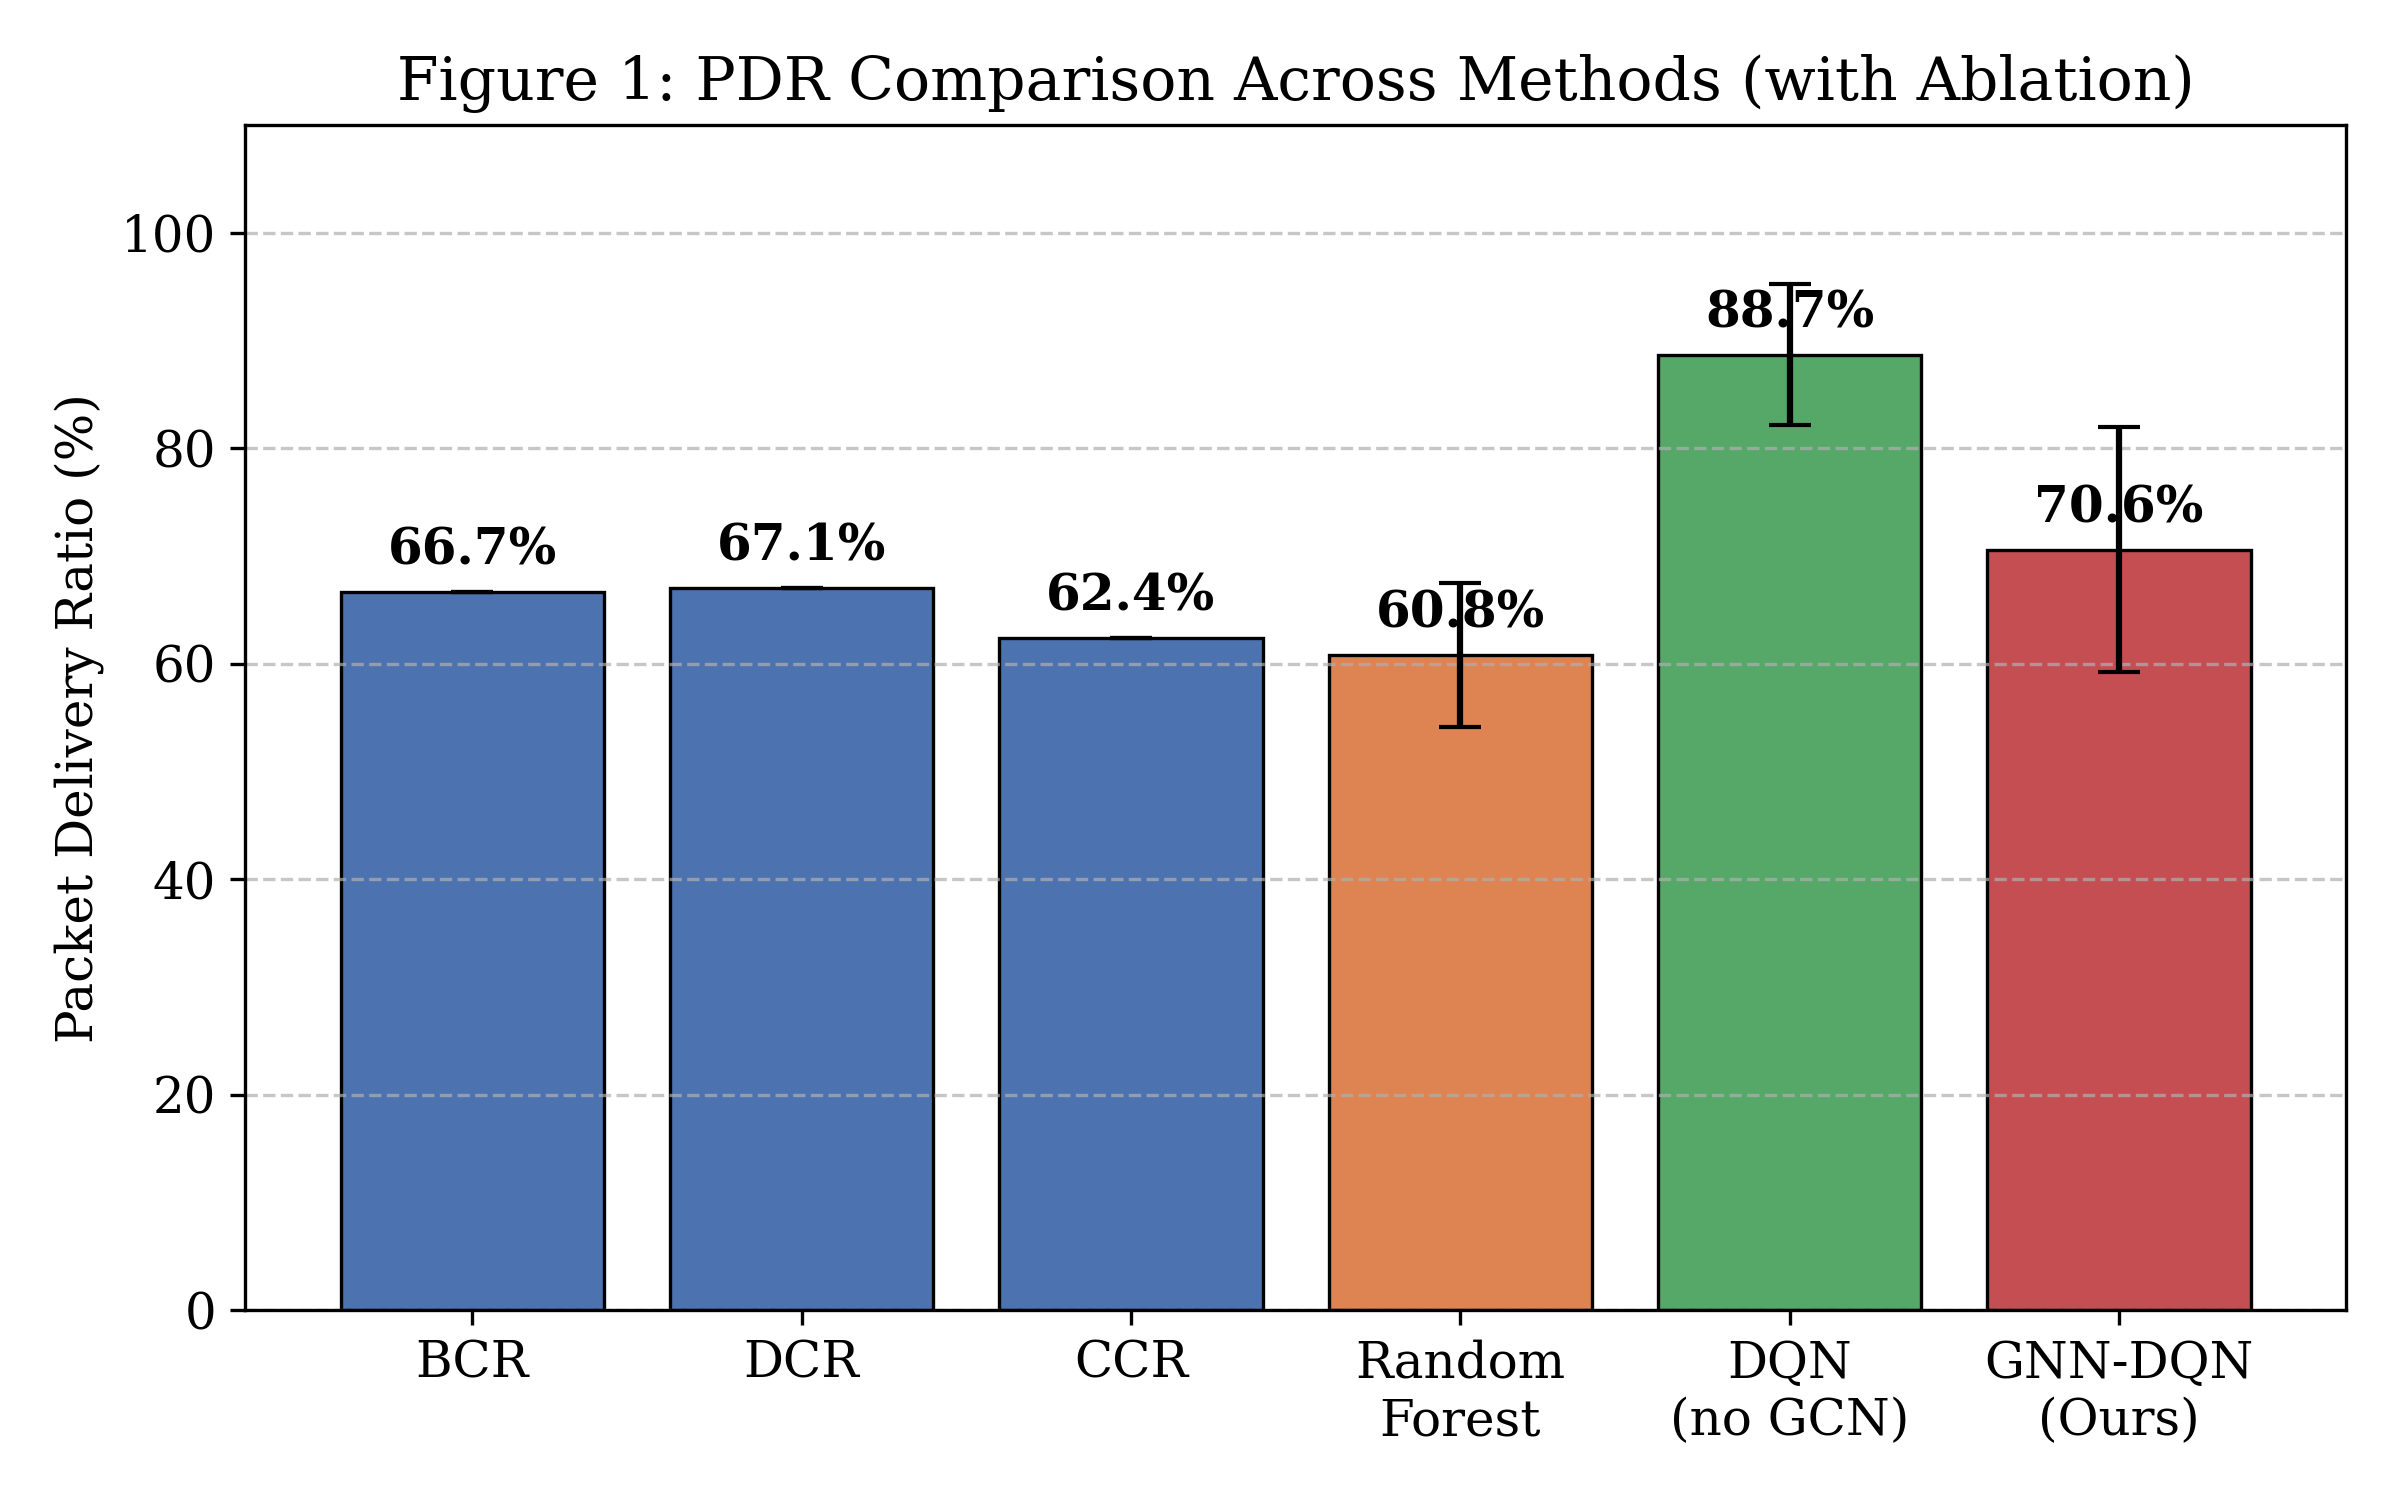
\includegraphics[width=0.48\textwidth]{fig1_pdr_comparison.png}
\caption{PDR comparison across all six methods. Error bars show the
standard deviation across seeds: 3 seeds for BCR/DCR/CCR, 10 seeds
for Random Forest, DQN (no GCN), and GNN-DQN.}
\label{fig:pdr}
\end{figure}

\begin{figure}[h]
\centering
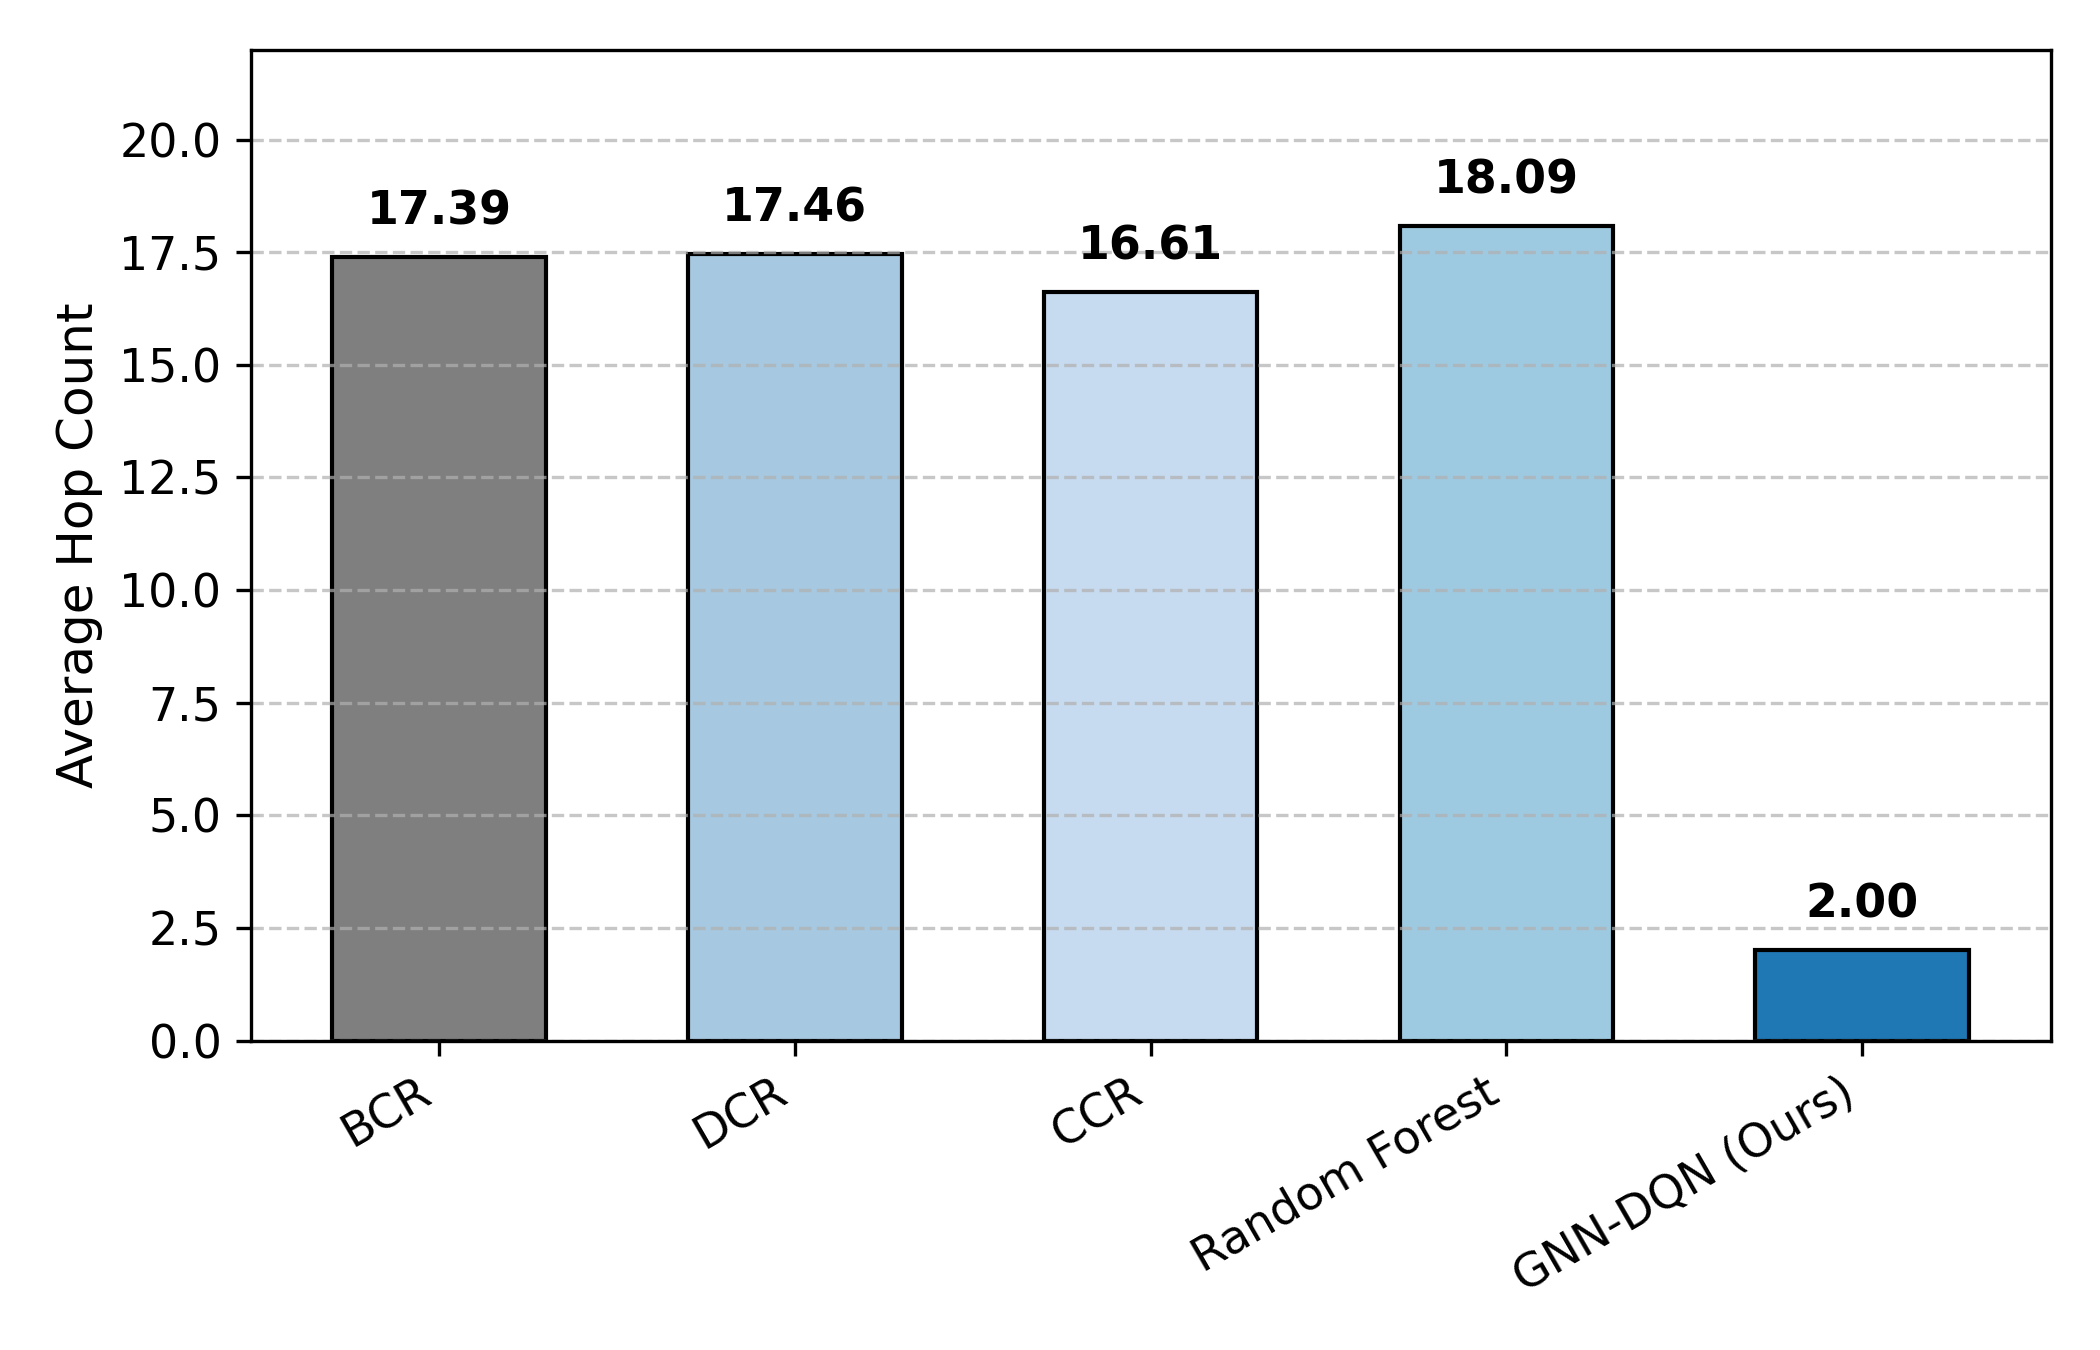
\includegraphics[width=0.48\textwidth]{fig2_hop_comparison.png}
\caption{Average hop count comparison from a single representative
100-episode evaluation run per method. GNN-DQN and DQN (no GCN)
achieve $<$2.5 hops vs.\ 16--18 for all other methods on this run.}
\label{fig:hops}
\end{figure}

\subsection{Statistical Analysis}
Across 10 independently generated topology instances, GNN-DQN
achieves mean PDR of $70.6\% \pm 11.33\%$ compared to
 $60.8\% \pm 6.68\%$ for RF. A Wilcoxon signed-rank test comparing
the two methods yields $p = 0.065$, a trend toward significance
that does not reach the conventional $\alpha = 0.05$ threshold; on
this sample size we cannot reject the null hypothesis of no
difference between the two methods' PDR distributions at the
conventional level. A paired t-test on the same data yields
 $p = 0.087$, consistent with this conclusion.

The observed mean difference (9.8 percentage points) is
nonetheless directionally consistent across most of the 10 seeds.
We attribute the gap between this practical effect size and the
non-significant statistical result primarily to GNN-DQN's
substantially higher variance ($\sigma = 11.33\%$ vs.\ $6.68\%$ for RF), which reflects topology-sensitivity of the learned
policy: its performance depends more on the specific topology
instance than RF's performance does. We report $p = 0.065$ exactly as observed rather than adjusting the framing, and we
explicitly do not run additional seeds solely to push this value
below 0.05, since doing so post hoc would constitute p-hacking.
A larger, pre-specified number of seeds is identified as future
work (Section~VI).

\subsection{Topology Generalisation}
As a preliminary test of generalisation beyond the training graph,
we evaluated the frozen GNN-DQN policy — with no fine-tuning — on
a single, previously unseen 80-node Erdős–Rényi graph (seed=99,
 $p=0.12$, 363 edges), using the same 100-episode evaluation
protocol as the single-run 50-node result. Under
this matched protocol, the frozen policy achieves 73.0\% PDR and
2.01 average hops on the unseen graph. Note that
this evaluation is based on the single-instance 81\%
training-topology result, not the 10-seed mean (70.6\%) used as
the primary result in Table~\ref{tab:results}; we use the
single-instance number here specifically because it matches the
unseen-graph evaluation's protocol.

\begin{figure}[h]
\centering
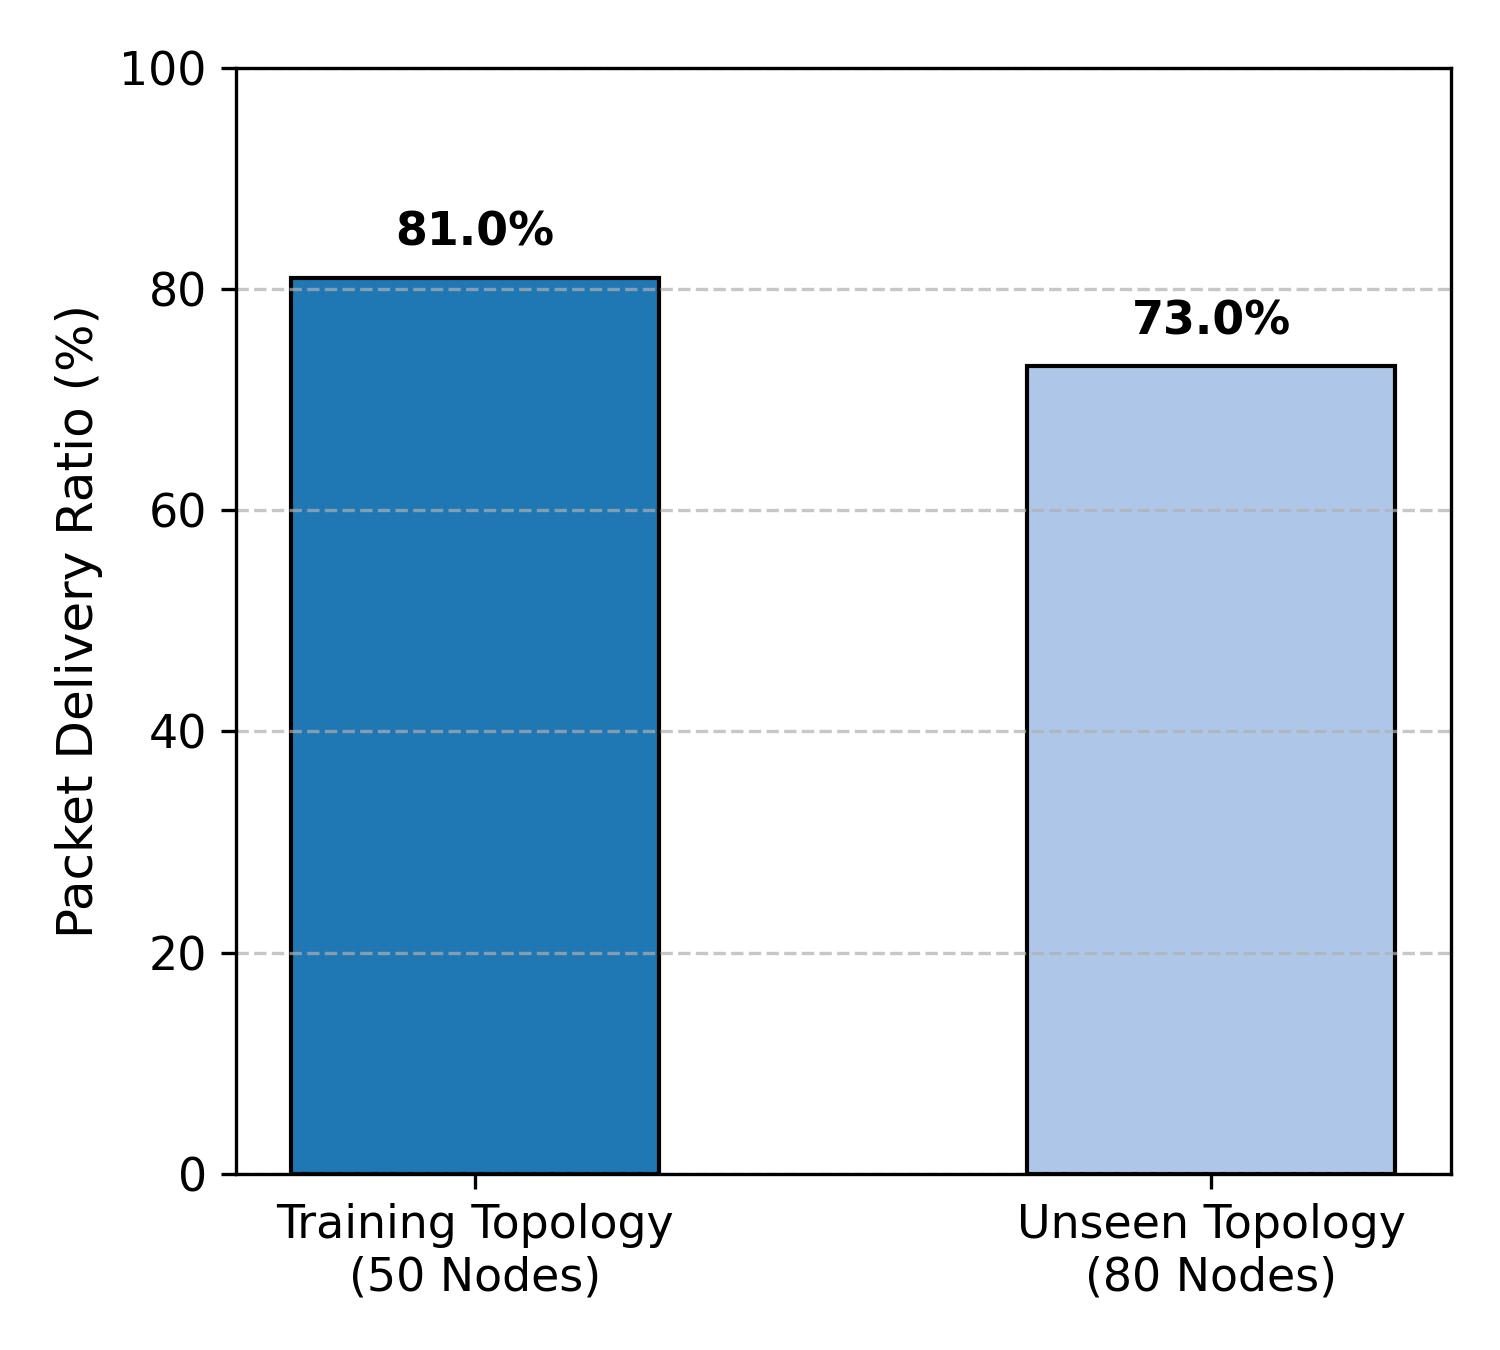
\includegraphics[width=0.40\textwidth]{fig3_generalisation.png}
\caption{GNN-DQN on the 50-node training-graph instance (81\% PDR,
single run) vs.\ a single unseen 80-node graph (73\% PDR, single
run), under matched 100-episode evaluation protocol.}
\label{fig:gen}
\end{figure}

This single result is consistent with the policy having learned
something beyond the exact training topology, since a policy that
had purely memorised training-graph specifics would be expected to
perform closer to random on a differently-sized, differently-seeded
graph. However, one unseen graph is not sufficient evidence of
general routing principles: we cannot rule out that this particular
graph happens to share favourable structural properties with the
training graph, nor characterise how performance varies across
different sizes, densities, or seeds. Furthermore, both the
GNN-DQN and plain DQN architectures output a fixed-size vector of
50 Q-values, meaning \emph{neither} model natively scales to
select nodes beyond the training set size; the 73\% PDR observed
here relies on environment-level fallback mechanisms for invalid
actions (substituting a real shortest-path hop whenever the
policy's chosen action is not a valid neighbour), rather than the
policy itself making a meaningful choice among the 80 available
nodes. We therefore do not have evidence, in the current
implementation, that the GCN encoder confers a genuine structural
generalisation advantage over the plain DQN. We report this result
as preliminary and identify systematic evaluation across multiple
unseen topologies — together with a transition to a per-node
Q-value architecture that would allow the action space to scale
with graph size — as necessary next steps before a generalisation
advantage can be claimed (Section~VI).

\subsection{Ablation Study}

To isolate the contribution of the GCN encoder, we trained a
plain DQN agent on the same 8-dimensional state vector used by
GNN-DQN, but with the GCNConv layers removed, evaluated across the
same 10 topology instances. The plain DQN achieved a mean PDR of
88.70\% ($\pm$6.53\%), significantly outperforming the 70.6\%
($\pm$11.33\%) achieved by GNN-DQN — a difference of 18.10
percentage points (Wilcoxon $p=0.0098$, $n=10$).
This indicates that raw centrality features provide a stronger
signal for next-hop selection on a fixed 50-node topology than
learned graph embeddings, largely due to information dilution from
global mean pooling, which averages node-specific structural
signals into a single graph-level representation. We note that
both the plain DQN and GNN-DQN share the same fixed
 $\text{Discrete}(50)$ output layer; consequently, we do not have
evidence that the GCN encoder provides an architectural
generalisation advantage over the plain DQN in its current form —
the 80-node result in Section~IV-C is preliminary and relies on
environment-level fallback for both architectures equally. This
finding identifies the mitigation of pooling dilution, together
with a move to per-node Q-value outputs so that the action space
scales with graph size, as a critical architectural refinement for
future work.

To determine whether the Plain DQN's advantage was solely due to
access to global centrality features, we conducted a secondary
ablation restricting both models to strictly local state
information (local degree and traffic load only, removing global
betweenness and closeness). Under this realistic local-knowledge
constraint, the Plain DQN again outperformed GNN-DQN, achieving
96.0\% PDR compared to GNN-DQN's 84.0\% across three topology
instances. This confirms that the performance degradation in
GNN-DQN is not merely due to redundant global inputs, but is
fundamentally caused by global mean pooling diluting node-specific
routing signals. Furthermore, it demonstrates that in dense,
static topologies, greedy degree-traffic heuristics learned by a
plain MLP are sufficient, rendering the structural learning of the
GCN encoder a liability in its current pooled architecture.

\section{Conclusion}
This paper presents GNN-DQN, a routing agent for opportunistic
networks that combines a Graph Convolutional Network encoder
with a Deep Q-Network policy. Evaluated across 10 independently
generated 50-node topology instances, GNN-DQN achieves a mean PDR
of 70.6\% $\pm$ 11.33\%, compared to 60.8\% $\pm$ 6.68\% for the
strongest baseline (Random Forest) — a 9.8 percentage-point
advantage that is directionally consistent but does not yet reach
conventional statistical significance ($p=0.065$). On a single
representative evaluation run, GNN-DQN reduces average hop count
to 2.0, an 88.9\% reduction versus 16--18 hops for all other
methods. On a single unseen 80-node topology, the frozen policy
achieves 73\% PDR, a preliminary result suggesting the policy is
not simply memorising the training graph, though broader
generalisation remains to be established across multiple
topologies, and both GNN-DQN and the plain-DQN ablation currently
share the same fixed 50-action limitation. An ablation study
reveals that a plain DQN significantly outperforms GNN-DQN on
fixed topologies ($p=0.0098$), indicating that global mean pooling
currently dilutes critical node-specific routing signals.

Limitations include high performance variance across seeds
($\sigma = 11.33\%$), a PDR advantage over the strongest baseline
that does not yet reach conventional statistical significance
($p = 0.065$), hop-count comparisons based on a single evaluation
run rather than a multi-seed average, a static-topology network
model that does not capture the connectivity dynamics of real
opportunistic networks, evaluation restricted to two graph
sizes (50 and 80 nodes), and the finding that the current GCN
architecture dilutes routing signals and shares the fixed
50-action limitation of the plain DQN, preventing true structural
generalisation from being claimed at this stage. Additionally, a
secondary ablation using only local features confirmed that the
GCN pooling dilution remains a liability even without global
centrality inputs (Plain DQN: 96.0\% vs.\ GNN-DQN: 84.0\%),
demonstrating that simple greedy heuristics outperform structural
learning in this architectural configuration. Future work will
address these directly: (1) evaluating hop counts and
generalisation across multiple independently generated topologies
of varying sizes and densities, (2) increasing the number of
training/evaluation seeds to obtain a statistically conclusive
comparison against the Random Forest baseline, (3) transitioning
to per-node Q-value architectures and attention-based pooling
(GAT) to preserve node-specific signals and enable native scaling
to unseen network sizes, (4) time-varying contact graphs to better
model genuine opportunistic connectivity, and (5) evaluation on
real-world contact traces (e.g.\ CRAWDAD).

\section*{Acknowledgment}
The authors thank Anil Carie for supervision and guidance
throughout this project.

\begin{thebibliography}{00}

\bibitem{wan2021}
Z. Wan, Y. Mahajan, B. W. Kang, T. J. Moore, and J. H. Cho,
``A Survey on Centrality Metrics and Their Network Resilience
Analysis,'' \textit{IEEE Access}, vol. 9,
pp. 104773--104819, 2021.

\bibitem{daly2007}
E. M. Daly and M. Haahr,
``Social network analysis for routing in disconnected
delay-tolerant MANETs,''
in \textit{Proc. ACM MobiHoc}, Montreal, QC, Canada,
2007, pp. 32--40.

\bibitem{raffin2021}
A. Raffin, A. Hill, A. Gleave, A. Kanervisto, M. Ernestus, and
N. Dormann, ``Stable-Baselines3: Reliable Reinforcement Learning
Implementations,'' \textit{Journal of Machine Learning Research},
vol. 22, no. 268, pp. 1--8, 2021.

\bibitem{babaria2025}
J. Babaria, K. Chokshi, V. S. A. Anala, R. Malik,
R. Thakkallapelly, and V. Chaudary,
``Graph Neural Network-Based Routing Optimization in
Large-Scale IoT Deployments,''
in \textit{Proc. 3rd Int. Conf. Advances in Computation,
Communication and Information Technology (ICAICCIT)},
2025, pp. 1505--1512.

\bibitem{manfredi2021}
V. Manfredi, A. P. Wolfe, B. Wang, and X. Zhang,
``Relational Deep Reinforcement Learning for Routing in
Wireless Networks,''
in \textit{Proc. IEEE 22nd Int. Symp. on a World of Wireless,
Mobile and Multimedia Networks (WoWMoM)}, 2021, pp. 159--168.

\bibitem{almasan2020}
P. Almasan, J. Suarez-Varela, A. Badia-Sampera, K. Rusek,
P. Barlet-Ros, and A. Cabellos-Aparicio,
``Deep Reinforcement Learning Meets Graph Neural Networks:
Exploring a Routing Optimization Use Case,''
\textit{arXiv:1910.07421}, 2020.

\bibitem{kipf2017}
T. N. Kipf and M. Welling, ``Semi-Supervised Classification with
Graph Convolutional Networks,'' in \textit{Proc. ICLR}, 2017.

\bibitem{mnih2015}
V. Mnih, K. Kavukcuoglu, D. Silver, A. A. Rusu, J. Veness,
M. G. Bellemare, A. Graves, M. Riedmiller, A. K. Fidjeland,
G. Ostrovski, S. Petersen, C. Beattie, A. Sadik, I. Antonoglou,
H. King, D. Kumaran, D. Wierstra, S. Legg, and D. Hassabis,
``Human-level control through deep reinforcement learning,''
\textit{Nature}, vol. 518, pp. 529--533, 2015.

\bibitem{schulman2017}
J. Schulman, F. Wolski, P. Dhariwal, A. Radford, and O. Klimov,
``Proximal Policy Optimization Algorithms,''
\textit{arXiv preprint arXiv:1707.06347}, 2017.

\bibitem{lent2022}
R. Lent, ``Dynamic routing in challenged networks with graph
neural networks,'' in \textit{Proc. 2022 IEEE Latin-American
Conference on Communications (LATINCOM)}, 2022, pp. 1--6.

\bibitem{das2025}
S. Das, N. NaderiAlizadeh, R. Mangharam, and A. Ribeiro,
``Opportunistic routing in communications networks via
learnable state-augmented policies,''
\textit{Frontiers in Communications and Networks}, 2026.

\end{thebibliography}

\end{document}